%----------- Terceiro Capítulo: Metodologia --------------

\chapter{Especificação} %(ou especifiação) 10 --- 20 pags

O \emph{software} a ser desenvolvido neste trabalho deverá fornecer uma ferramenta flexível de degradação de vídeo digital e também de avaliação subjetiva e objetiva das mídias.
Neste capítulo serão apresentados os requisitos de tal sistema, assim como as especificações de desenvolvimento, arquitetura e funcionamento.

\section{Análise de Requisitos}

A análise de requisitos é parte fundamental de qualquer projeto, buscando atender da melhor forma as necessidades dos futuros usuários.
Esta sessão descreve os requisitos levantados após o estudo e planejamento da ferramenta.

\subsection{Requisitos Funcionais}

Requisitos funcionais são aqueles determinados pelas funcionalidades exigidas do sistema, ou seja, as ações que se espera que o sistema execute. 
Foram levantados os seguintes requisitos funcionais:

\begin{itemize}
	\item O \emph{software} deverá possuir ferramentas de degradação de vídeos digitais.
	\item O \emph{software} deverá possuir uma ferramenta de simulação de transmissão \emph{streaming}.
	\item O \emph{software} deverá ser capaz de criar e gerenciar sessões de avaliação subjetiva.
	\item O \emph{software} deverá ser capaz de exibir os vídeos existentes na base de dados.
	\item O \emph{software} deverá exibir os resultados das avaliações objetivas e subjetivas de forma gráfica.
\end{itemize}

\subsection{Requisitos Não-Funcionais}

Requisitos não-funcionais são aqueles ditados por restrições ou exigências de qualidade ou de operação, tais como performance, segurança ou tecnologias envolvidas.
Abaixo se encontram os requisitos não funcionais levantados:

% TODO dividir por categorias: padronização, usabilidade, tecnologias envolvidas.

\begin{itemize}
	\item As ferramentas de degradação e métricas objetivas deverão operar sobre vídeos em formato YUV planificado com subamostragem 4:2:0.
	\item A ferramenta de simulação deverá operar sobre vídeos no formato \sigla{H.262}{Padrão de compressão de vídeo digital também conhecido MPEG-2 Part 2} encapsulados em um Transport Stream (\sigla{TS}{Transport Stream}).
	\item O sistema deve fornecer documentação detalhada de auxílio ao uso das ferramentas.
	\item A ferramenta de exibição deverá ser executada em um sistema capaz de prover um \emph{display} com resolução igual ou maior que a dos vídeos a serem exibidos.
	% TODO verificar a versão da JRE necessária para rodar a interface
	\item A interface gráfica do sistema necessita que haja um \emph{Java Runtime Environment} (\sigla{JRE}{Java Runtime Environment}) instalado no sistema operacional.
\end{itemize}

\section{Especificações do Software}

Esta seção tem o propósito de descrever a arquitetura proposta para o SASQV2, assim como abordar as diferentes linguagens e bibliotecas que ajudam a integrar o programa.

\subsection{Arquitetura do Sistema}

Por se tratar da continuação do desenvolvimento do projeto SASQV, este trabalho reutiliza e adapta grande parte dos componentes existentes no trabalho original. 
A Figura \ref{fig:arquitetura} mostra uma comparação entre as visões gerais de ambos os projetos. A diferença mais notável entre estas arquiteturas é a separação dos componentes de serviço e o de ferramentas, além de também recriar o componente de interface gráfica para melhor atender às necessidades do sistema. 
Mais detalhes sobre cada componente da arquitetura são descritos em seções específicas a seguir.

\begin{figure}[!htb]
	\centering
	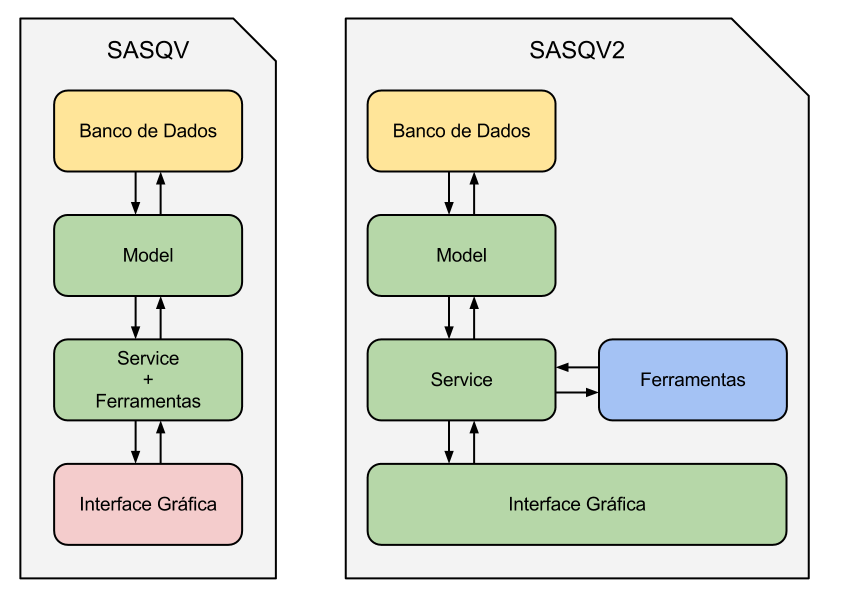
\includegraphics[width=0.9\textwidth]{./imgs/arquitetura.png}
	\caption{Visão geral das arquiteturas dos sistemas SASQV e SASQV2.}
	\label{fig:arquitetura}
	\fonte{Autoria Própria.}
\end{figure}

\subsubsection{Banco de Dados}

O componente banco de dados foi completamente reaproveitado, seguindo as mesma especificações do SASQV. 
O Sistema Gerenciador de Banco de Dados (\sigla{SGBD}{Sistema Gerenciador de Banco de Dados}) escolhido foi o MySQL, atualmente o SGDB \emph{open source} mais utilizado no mundo \cite{mysqlmarket}.
O MySQL foi lançado e desenvolvido em 1995 pela empresa Sueca MySQL AB, atualmente incorporada pela Oracle Corporation, na forma de um SGDB que fornece um servidor multi-usuários para bancos de dados relacionais \cite{wikipediamysql}. 
Juntamente do MySQL também é utilizado o MySQL Workbench, uma ferramenta distribuida pela Oracle que concilia um cliente MySQL, uma ferramenta de \emph{Database Moddeling} e um administrador de servidor MySQL. 
A versão \emph{open source} de ambas as ferramentas é distribuída sob a licensa GNU General Public License (\sigla{GPL}{General Public License}).

O modelo Entidade-Relacionamento (\sigla{ER}{Entidade-Relacionamento}) é o mesmo utilizado pelo SASQV, como mostrado na Figura \ref{fig:diagramaER}.

\begin{figure}[!htb]
	\centering
	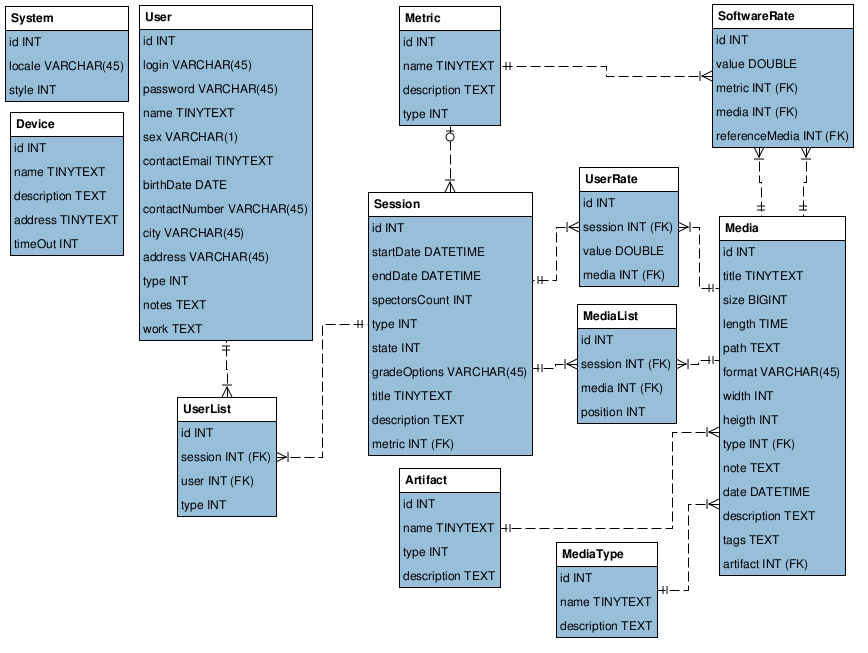
\includegraphics[width=0.9\textwidth]{./imgs/diagramaER.png}
	\caption{Diagrama Entidade-Relacionamento do SASQV2}
	\label{fig:diagramaER}
	\fonte{Autoria Própria}
\end{figure}

\subsubsection{Model}

O componente Model presente no SASQV2 também foi reaproveitado inteiramente do SASQV, cabendo apenas algumas adições. Este componente consiste na implementação de um mapeamento objeto-relacional (\sigla{MOR}{Mapeamento Objeto Relacional}) por meio da biblioteca Hibernate. 
O Hibernate teve seu desenvolvimento iniciado em 2001 por Gavin King, com o objetivo de melhorar as ferramentas de persistência existentes na plataforma Java \cite{hibernateHistory}, e é atualmente distribuído sob a licensa GNU Lesser General Public License (\sigla{LGPL}{Lesser General Public License}) \cite{hibernateAbout}.
A biblioteca provê um mapeamento flexível entre objetos Java e tipos SQL, eliminando a custosa necessidade de processamento manual e repetitivo de listas de resultados obtidas via SQL e JDBC.
Estima-se que até cerca de 30\% do código de uma aplicação possa ser poupado utilizando MOR, além de incrementar a portabilidade do sistema suportando diversas implementações de Bancos de Dados SQL em troca de um pequeno \emph{overhead} de performance.

\subsubsection{Service}
\subsubsection{Ferramentas}
\subsubsection{Interface Gráfica}
\subsection{Linguagens}
\subsection{Bibliotecas}
\subsection{Diagramas de Caso de Uso}
\section{Considerações}
